\documentclass{article}
\usepackage{amsmath,amssymb,array}
\textheight 21cm
\textwidth 15cm
\usepackage{bm}
\usepackage{diagbox}
\usepackage{epsfig}
\usepackage{indentfirst}
\usepackage[colorlinks=true, linkcolor=red, citecolor=blue,CJKbookmarks=true]{hyperref}
\usepackage[top=1in, bottom=1in, left=1.25in, right=1.25in]{geometry}

\def\blue#1{{\textcolor{blue}{#1}}} % blue color
\def\red#1{{\textcolor{red}{#1}}} % red color
\newcommand{\bt}{\beta}
\newcommand{\ep}{\epsilon}
\newcommand{\f}{\frac}
\newcommand{\lt}{\left}
\newcommand{\n}{\nonumber}
\newcommand{\p}{\partial}
\newcommand{\rd}{{\rm d}}
\newcommand{\rt}{\right}
\newcommand{\ve}{\varepsilon}
\newcommand{\vp}{\varphi}
\newcommand{\arXg}[1]{\href{http://arxiv.org/abs/#1}{{\ttfamily arXiv:#1[gr-qc]}}}
\newcommand{\arXh}[1]{\href{http://arxiv.org/abs/#1}{{\ttfamily arXiv:#1[hep-th]}}}

\def\TeV{\mathrm{TeV}} % TeV
\def\GeV{\mathrm{GeV}} % GeV
\def\MeV{\mathrm{MeV}} % MeV
\def\keV{\mathrm{keV}} % keV
\def\kpc{\mathrm{kpc}} % keV
\def\eV{\mathrm{eV}} % keV
\def\um{\mu\mathrm{m}} % keV
\def\cm{\mathrm{cm}} % keV

\begin{document}

\title{Reply to the Comments of Referee} \maketitle \date{}

\begin{flushleft}
\textbf{Title:} Prospect for dark matter self-annihilation signatures from dwarf galaxies by LHAASO

\textbf{Manuscript ID:} DD12310/He

\textbf{Authors:} Dong-Ze He, Xiao-Jun Bi, Su-Jie Lin, Peng-Fei Yin and Xin Zhang
\end{flushleft}
\vspace{3mm}




We deeply appreciate the referee for providing constructive comments on our manuscript.
Taking all the comments into account, we have once again submitted a revised version of our manuscript. Revised portion are marked in red in the attached PDF file. The main responds to the comments and questions are listed as follows.


\begin{quote}
\emph{Thank you for improving the manuscript and addressing most of the issues raised. I have one comment related to the absorption and one request for a major revision related to the
sensitivity calculation.}


\emph{On the CMB absorption. Just below 100 TeV, the CMB absorption will dominate even above the interstellar radiation field (specifically, when considering high Galactic latitude line of
sight). The authors propose a simplified calculation where the consider only the average photon energy of the CMB. However, a more careful treatment shows the following picture: 
\begin{figure*}[!h]\centering
  \includegraphics[width=0.60\textwidth]{referee.png}
%\caption{The revised CMB absorption following Gould $\&$ Schreder (1967).}
\label{re}
\end{figure*}}

\emph{The Eq. $6$ is technically correct but assumes that the CMB is monoenergetic and anisotropic. Instead, a treatment already proposed by Gould $\&$ Schreder (1967) provides the correct attenuation factor. Eq. $7$ is certainly not applicable given that the line of sight towards dwarf galaxies is not passing through a large amount of interstellar radiation field given the high Galactic latitude (with the exception of Sgr Dw.). In summary, the conclusion should be that the CMB attenuation starts to be relevant just below 100 TeV for the more distant galaxies, below that energy and for galaxies with small value of the galactic latitude, additional absorption from the interstellar radiation field takes place but can safely be ignored.}
\end{quote}

\textbf{Reply:} We thank the referee for such a detailed calculation and careful comment on this issue. We totally agree that it is quite necessary to calculate the CMB attenuation in order to thoroughly clarify the absorption effect. Therefore, we have added an appendix in the revised manuscript to discuss this issue, in which the detailed equation from Gould $\&$ Schreder (1967) \cite{Gould:1967zzb} is introduced and an estimation on the absorption is given. As we re-calculated the absorption, we accidentally found that there are some typos in the Eq.10, Eq.13b and Eq.19b of Gould $\&$ Schreder (1967) \cite{Gould:1967zzb}. In fact, these equations ought to be
\begin{align*}
  \bar{\varphi}[s_0]&=\frac{1+\beta_0^2}{1-\beta_0^2}\ln(\omega_0) - \dots + 4\ln(\omega_0)\ln(\omega_0+1) - \textcolor{red}{4L(\omega_0)},\\
  \bar{\varphi}[s_0]&=(4/3)(s_0-1)^{3/2} + (16/5)(s_0-1)^{5/2} + (132/35)(s0 - 1)^{7/2} + \dots (s_0-1\ll1),\\
  f(\nu)&\rightarrow\sqrt{\pi}e^{-\nu}(\sqrt{\nu}+6/\sqrt{\nu}\dots) (\nu\gg1).
\end{align*}
We have compared the results from the corrected equations with the totally numerical result of Eq.(8), Eq.(9), and Fig.2 in Gould $\&$ Schreder (1967) to ensure the correctness.
As a result, the final estimated absorption is a bit looser than the referee's figure, and the TeV photons are unlike to be affected even for a distance as far as 1 Mpc (see Fig. \ref{op}).
\begin{figure*}[htbp]
  \centering
  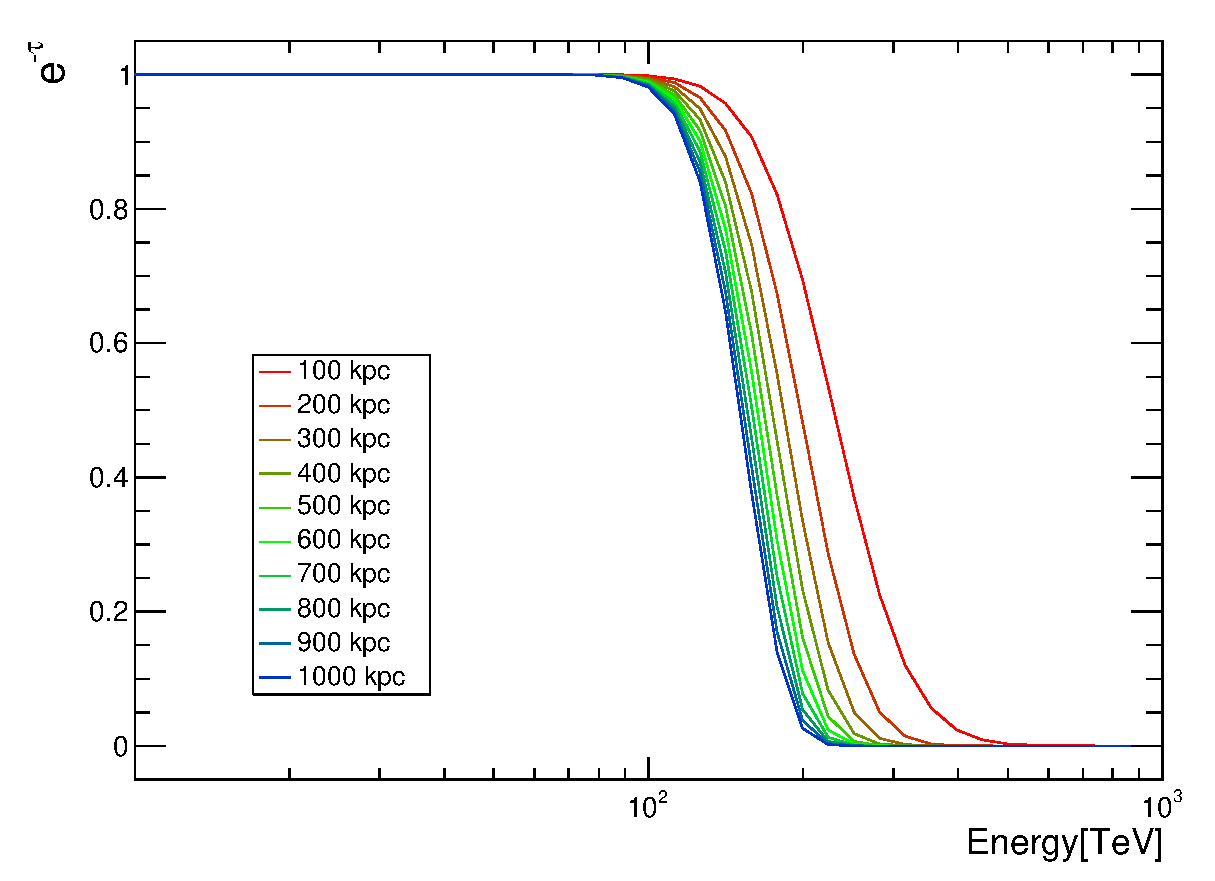
\includegraphics[width=0.60\textwidth]{figs/opacity.eps}
  \caption{The revised CMB absorption in light of the results of Gould $\&$ Schreder (1967).}
  \label{op}
\end{figure*}

As for the interstellar radiation field (ISRF), we totally agree with the referee that it can be safely ignored.
Since the detailed calculation of the ISRF is complex and beyond the topic of this paper, in the added appendix of the revised version we just introduce the results from a relevant paper~\cite{Zhang:2005tp} to demonstrate that the contribution of ISRF to the absorption could also be neglected.

What's more, in the previous version we used 100 TeV as the critical energy.
That is in fact over conservative, as the most energetic gammas considered in this work would be $\sim20\,\TeV$ for the WCDA.
We have also corrected this point in the updated discussion.

\begin{quote}
\emph{Concerning the calculation of the sensitivity. Thanks for clarifying and providing the reference to $[3]$ (ICRC 2017 conference proceedings). As the approach used for the calculation becomes more clear, there are more issues that need to be considered or discussed.}

\emph{Let’s start with the collection areas (taken from arXiv:1905.02773, Fig. $46$):}

\emph{The collection areas are obtained for a cut $N_{\rm fit} \geq 10$. For the calculation of the background and signal, the authors assume a constant value of $\varepsilon_{p} = 0.278\%$ (I still wonder why the precision of three digits is assumed?) for the proton efficiency and $\varepsilon_{\gamma} = 40\%$. This corresponds to a $Q = 7.6$. While in $[3]$, the Q-factor for the interval $10 \leq N_{\rm fit} \leq 20$ is given to be closer to $4.6$. In principle, the assumed effective areas and the gamma/hadron separation are not consistent with each other. I understand that a value of \,$7.6$ for the Q-factor is conservative for larger values of $N_{\rm fit}$ , however, the authors assume a collection area for $N_{\rm fit}$ above $10$. I understand that the focus of the work lies at WIMPs above TeV-energies. But even for a TeV-mass, the signal is dominated by events at much lower energies closer to the lower interval of $N_{\rm fit}$.}

\emph{Furthermore, the authors use a point-spread function that is not published. In principle, they could use the one quoted in the white paper (Fig. $45$). However, that one is again obtained for $N_{\rm fit} > 20$.}
\end{quote}

\textbf{Reply:} We thank the referee for such a critical question that we have not clarified.
In the previous calculation, we focus on the gamma photons with energies higher than 300 GeV.
In the present stage, we have inverted the concentration to the gamma photons with energies higher than 700 GeV.
This energy range corrsponds to $N_{\rm fit} > 20$ as shown in Ref. \cite{Zha:2017vcs}, thus most of the events with $N_{\rm fit} < 20$ are actually ignored here.
Therefore, the difference of the $N_{\rm fit}$ cut between the effective areas~\cite{Bai:2019khm} and the gamma/hadron separation has no effect on our calculation in the updated manuscript.

Besides, for the angular resolution (point-spread function), as suggested by the referee, we change to use the one described in the Fig. 45 of LHAASO Science White Paper \cite{Bai:2019khm}.

%It should be stressed that,  the inconsistent assumptions of the trigger multiplicity $N_{\rm fit}$ between the effective area with the gamma/hadron separation as well as the point-spread function can not influence the practical calculations significantly.

As we utilize the new point-spread function and reconsider the gamma photon's energy range in the study, the main results of calculation, especially in the low energy range, has significantly changed, which can be find in the revised version of our manuscript  (i.e., Fig. 2 and Fig. 3 in the manuscript). 

We have added these discussions in the revised manuscript.
\begin{quote}
\emph{My apologies for being persistent on this point, but I can not recommend the publication of these results which are based upon inconsistent (collection area and gamma/hadron separation) and non-published (point-spread function) assumptions for the calculation of the sensitivity. Since this is at the heart of the study, I believe these points need to be clarified in a consistent manner before proceeding with the publication or at least addressing the effect of the inconsistent assumptions.}
\end{quote}

\textbf{Reply:} Finally, we emphasize that the inconsistency of the trigger multiplicity $N_{\rm fit}$ between collection area and gamma/hadron separation has been resolved. Also, we have inverted the utilization of the point-spread function to a published result as described in the Science White Paper \cite{Bai:2019khm}. We hope the referee would find that our research results are at present reasonable and reliable. 
\vskip 1cm

In summary, we have already carefully revised our manuscript according to the referee's comments. We hope the above answers would satisfy the referee and our work would become suitable for the publication in Physical Review D. Thanks a lot!

\bibliographystyle{unsrt}
\bibliography{reference}


\end{document}
